\documentclass[12pt]{article}

%% FONTS
%% To get the default sans serif font in latex, uncomment following line:
 \renewcommand*\familydefault{\sfdefault}
%%
%% to get Arial font as the sans serif font, uncomment following line:
%% \renewcommand{\sfdefault}{phv} % phv is the Arial font
%%
%% to get Helvetica font as the sans serif font, uncomment following line:
% \usepackage{helvet}
\usepackage[small,bf,up]{caption}
\renewcommand{\captionfont}{\footnotesize}
\usepackage[left=1in,right=1in,top=1in,bottom=1in]{geometry}
\usepackage{graphics,epsfig,graphicx,float,subfigure,color}
\usepackage{amsmath,amssymb,amsbsy,amsfonts,amsthm}
\usepackage{url}
\usepackage{boxedminipage}
\usepackage[sf,bf,tiny]{titlesec}
 \usepackage[plainpages=false, colorlinks=true,
   citecolor=blue, filecolor=blue, linkcolor=blue,
   urlcolor=blue]{hyperref}
\usepackage{enumitem}
\usepackage{verbatim}
\usepackage{tikz,pgfplots}

\newcommand{\todo}[1]{\textcolor{red}{#1}}
% see documentation for titlesec package
% \titleformat{\section}{\large \sffamily \bfseries}
\titlelabel{\thetitle.\,\,\,}

\newcommand{\bs}{\boldsymbol}
\newcommand{\alert}[1]{\textcolor{red}{#1}}
\setlength{\emergencystretch}{20pt}

\begin{document}

\begin{center}
  \vspace*{-2cm}
{\small MATH-GA 2012.001 and CSCI-GA 2945.001, Georg Stadler \&
  Dhairya Malhotra (NYU Courant)}
\end{center}
\vspace*{.5cm}
\begin{center}
\large \textbf{%%
Spring 2019: Advanced Topics in Numerical Analysis: \\
High Performance Computing \\
Assignment 6 (due May 13, 2019) }
\end{center}

\vspace*{.5cm}
\begin{center}
\Large \textbf{Terrence Alsup}
\end{center}


\vspace{1cm}
All runs were done on Prince with 64 cores by running an interactive session with the command:\\
\begin{center}
\texttt{srun --nodes=8 --ntasks-per-node=8 --pty /bin/bash}
\end{center}
The processors used were Intel(R) Xeon(R) CPU E5-2690 v4 @ 2.60GHz.  The Python file \texttt{timing\_plotter.py} can be run to plot the strong and weak scaling timings for the 2D Jacobi method.  This files requires matplotlib which is included in Anaconda3.


% ****************************
\begin{enumerate}
% --------------------------
\setcounter{enumi}{-1}

  
\item {\bf Final project update.} Anya and I have finished most of the 1D parallel implementation of KMC using MPI.  We have a bug that is causing the program to hang that we are still working on.  The serial code for 1D as well as 2D has already been completed.  Next we will move to the 2D parallel case which should be a straightforward extension given our 1D implementation.  Hopefully by the end of this week we will have moved on to performing scalability tests.




\item {\bf MPI-parallel two-dimensional Jacobi smoother.} \\
The 2D Jacobi smoother is implemented in the file \texttt{jacobi2D-mpi.cpp}.  We assume that the number of cores used is a power of $4$ (i.e. $4^j$ for some $j = 0,1,2,\ldots$), and that the size of the matrix is $N\times N$ with $N = 2^j N_l$.  Figure~\ref{fig:weak_scaling} below shows the timings as we increase the number of processors with a fixed amount of work per processor.  Figure~\ref{fig:strong_scaling} shows the timings as we increase the number of processors for a fixed amount of work.


\begin{figure}[H]
\begin{center}
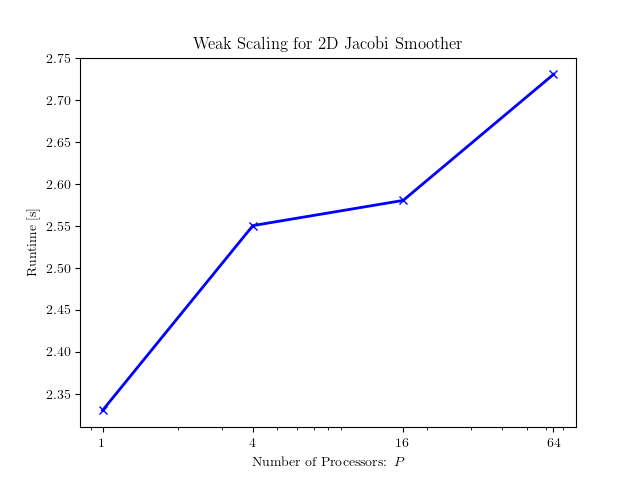
\includegraphics[width=5in]{weak_scaling.png}
\end{center}
\caption{A weak scaling study for the MPI implementation of the 2D Jacobi smoother.  We have fixed $N_l = 400$ and do $10^4$ Jacobi iterations.  We see that increasing the number of processors slightly increases the runtime, mainly due to more memory transfers.}
\label{fig:weak_scaling}
\end{figure}

\begin{figure}[H]
\begin{center}
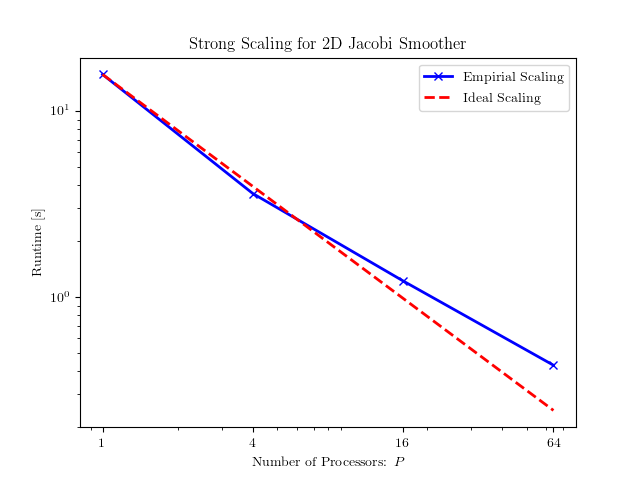
\includegraphics[width=5in]{strong_scaling.png}
\end{center}
\caption{A strong scaling study for the MPI implementation of the 2D Jacobi smoother.  We have fixed $N = 1000$ and do $10^4$ Jacobi iterations.  We see that increasing the number of processors decreases the runtime and the scaling is approximately a factor of $1/4$-th, which is ideal.}
\label{fig:strong_scaling}
\end{figure}

\item {\bf Parallel sample sort.}  
 
The MPI implementation of sample sort is in the file \texttt{ssort.cpp}.  Table~\ref{table:sort_times} below shows the timings for different $N$ on Prince with 64 cores.

\begin{table}[H]
\begin{center}
\begin{tabular}{l | r }
$N$ & Runtime [s] \\
\hline
$10^4$ & 0.82\\
$10^5$ & 0.84\\
$10^6$ & 1.13
\end{tabular}
\end{center}
\caption{The runtime [s] for sample sort with different $N$.  For $N =10^4$ and $10^5$ the results are roughly the same indicating that most of the time is spent transferring memory between the processors.  $N = 10^6$ is large enough so that time for memory transfers is no longer dominant.}
\label{table:sort_times}
\end{table}


\end{enumerate}
\end{document}
